\large{
\section{Struttura dati}
Prima ancora di mostrare l'interfaccia e le scelte progettuali applicate è necessario definire con chiarezza la struttura dati con cui l'utente andrà a lavorare ricordando infatti che una visualizzazione per buona che sia non ha valore senza la possibilità di analisi del dato di cui ne è la rappresentazione.
Ritornando al capitolo relativo allo stato dell'arte, si è definito un grafo clusterizzato $C$ come una coppia $<G,T>$ in cui $G$ è l'underlying graph definito dalla coppia $<V,E>$ rispettivamente di nodi ed archi e $T$ è l'inclusion tree. Alla base di questo e seguendo quanto detto nel capitolo due relativo agli oggetti scelti per la struttura dati, vi è la rappresentazione del grafo clusterizzato così come mostrato nella figura \figurename~\ref{fig:cgraphClass}. Un oggetto \textit{clusteredGraph} è definito mediante un oggetto relativo all'underlying graph ed uno relativo all'inclusion tree.\\
Come si nota un oggetto \textit{UnderlyingGraph} è definito mediante una primitiva String che ne rappresenta l'etichetta e mediante due oggetti Map: Map<number,Node> in cui sono elencati tutti i nodi di cui è composto il grafo e Map<number,Edge> per gli archi. 
\begin{figure}[!htb]
	\begin{center}
		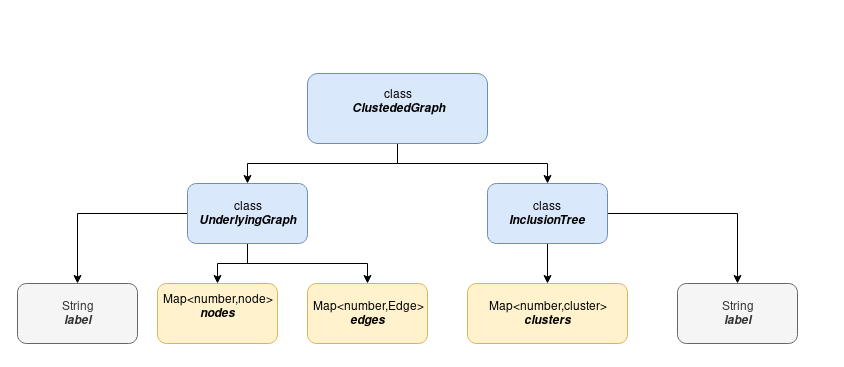
\includegraphics[width=1 \linewidth]{figure/cgraphClass}
	\end{center}
	\caption{Oggetto clusteredGraph\label{fig:cgraphClass}}
\end{figure}
Andando poi a ritroso nelle definizioni, nella figura \figurename~\ref{fig:nodeClass} è mostrato l'oggetto Nodo. Esso può essere definito mediante un costruttore di tre valori:
\begin{itemize}
	\item \textbf{label} di tipo primitivo String che ne definisce l'etichetta;
	\item \textbf{id} un numero, identificativo insieme alla sua etichetta ma ancor più personale, del nodo in questione;
	\item \textbf{rotationScheme} di tipo Set<number> in cui vengono salvati tutti gli ID degli archi che hanno quel nodo come nodo di partenza o di destinazione.
\end{itemize}
Ogni nodo è un elemento fondamentale dell'underlying graph da visualizzare e connettere.
\begin{figure}[!htb]
	\begin{center}
		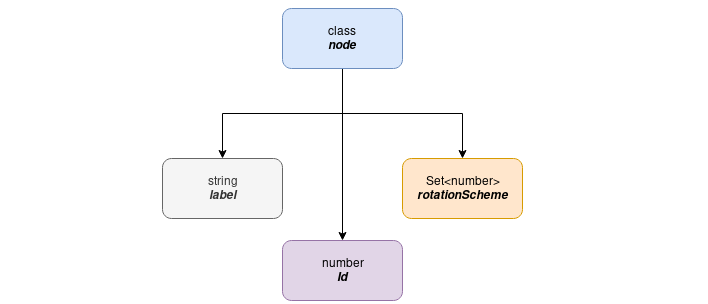
\includegraphics[width=1 \linewidth]{figure/nodeClass}
	\end{center}
	\caption{Oggetto nodo del underlying graph\label{fig:nodeClass}}
\end{figure}
Restando sempre nella creazione dell'oggetto \textit{UnderlyingGraph} del grafo clusterizzato risulta, esattamente come per l'oggetto \textit{node}, necessario fornire la definizione dell'oggetto relativo agli archi.
La classe dell'oggetto \textit{Edge} rappresentata in \figurename~\ref{fig:edgeClass} è definita mediante una stringa e tre valori numerici. La prima si riferisce all'etichetta dell'arco e non necessariamente dovrà essere unica, i valori numerici invece fanno riferimento all'id dell'arco, necessario non solo per unificare l'arco creato ma anche per essere inserito nel Set<number> \textit{rotationScheme} del nodo che lo vedrà collegato. Ogni arco collegherà poi un nodo di inizio fino ad un nodo di arrivo anche se non in maniera orientata, in quanto il nodo di inizio e il nodo di fine arco saranno solamente quelli relativi a dove l'utente vorrà che la visualizzazione dell'arco inizi e finisca. Per questo ogni elemento della classe arco avrà due valori numerici \textit{source} che conterrà l'id del nodo di partenza e \textit{target} con l'id del nodo di destinaione. 
\begin{figure}[!htb]
	\begin{center}
		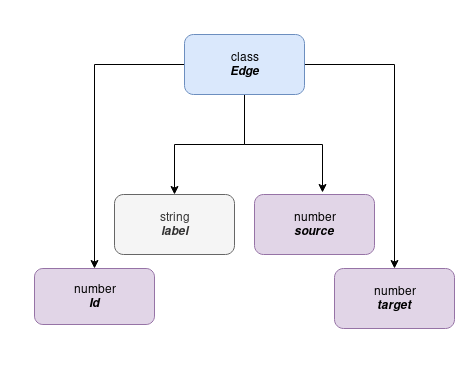
\includegraphics[width=1 \linewidth]{figure/edgeClass}
	\end{center}
	\caption{Oggetto arco dell'undelying graph\label{fig:edgeClass}}
\end{figure}

Termina la definizione della classe \textit{UnderlyingGraph} si può passare a quella della classe \textit{InclusionTree}. Ogni oggetto appartenente a questa classe possiede una etichetta definita come tipo String, esattamente come per la sua controparte grafo, e una lista contenente i cluster che fanno parte dell'albero di inclusione, di tipo Map<number,Cluster>.
Andando a ritroso anche in questa struttura si vuol definire di seguito la classe \textit{Cluster}.
Un oggetto \textit{cluster} come mostrato nella figura \figurename~\ref{fig:clusterClass} è definito mediante un costruttore con cinque attributi di seguito riportati:
\begin{itemize}
	\item \textbf{label} di tipo String che ne rappresenta l'etichetta;
	\item \textbf{level} di tipo number, definisce il livello ovvero la profondità a cui il cluster si troverà all'interno dell'albero di inclusione;
	\item \textbf{cildren} di tipo Set<number> e che contiene gli id dei cluster di profondità superiore collegati con il cluster di interesse, ovvero i suoi figli;
	\item \textbf{parents} di tipo Set<number> contenente gli id dei cluster di profondità inferiore e che sono collegati al cluster di interesse, ovvero i suoi genitori;
	\item \textbf{nodes} di tipo Set<number> contenente gli id dei nodi che sono contenuti all'interno del cluster
\end{itemize}

\begin{figure}[!htb]
	\begin{center}
		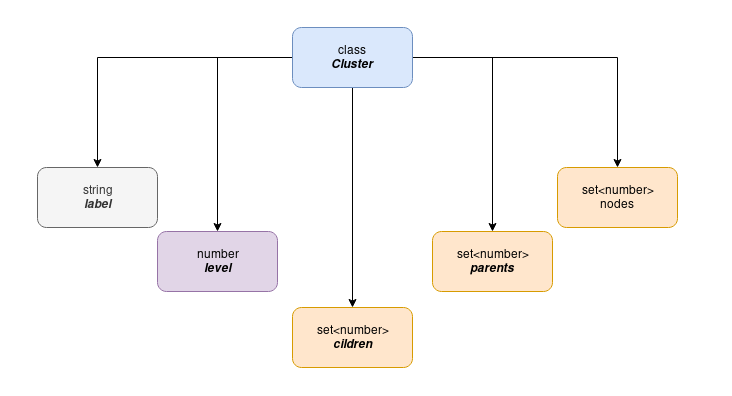
\includegraphics[width=1 \linewidth]{figure/clusterClass}
	\end{center}
	\caption{Oggetto cluster dell'inclusion Tree\label{fig:clusterClass}}
\end{figure}

\section{Log-in ed inizializzazione}
Al momento del log-in iniziale l'utente si troverà la schermata mostrata nella \figurename~\ref{fig:interfaccia}. Come è possibile notare da subito sono stati utilizzati molti dei principi di visualizzazione visti in precedenza cominciando dall'impiego e della posizione dei bottoni necessari per le interazioni dell'utente. È stato lasciando poi grande spazio per quanto concerne il piano di lavoro principale che come si vedrà successivamente rimarrà inalterato anche cambiando l'interfaccia utilizzata. Anchel'impiego di colori caldi quale il blu rispetto al piano di lavoro di colore chiaro lascia intendere la maggiore importanza ed evidenza che deve avere il secondo rispetto al resto dell'interfaccia. Ogni qualvolta l'utente vorrà interagire con il sistema sarà sufficiente cliccare una delle operazioni, che saranno viste nel capitolo successivo, per poter avere una risposta.
\begin{figure}[!htb]
\begin{center}
	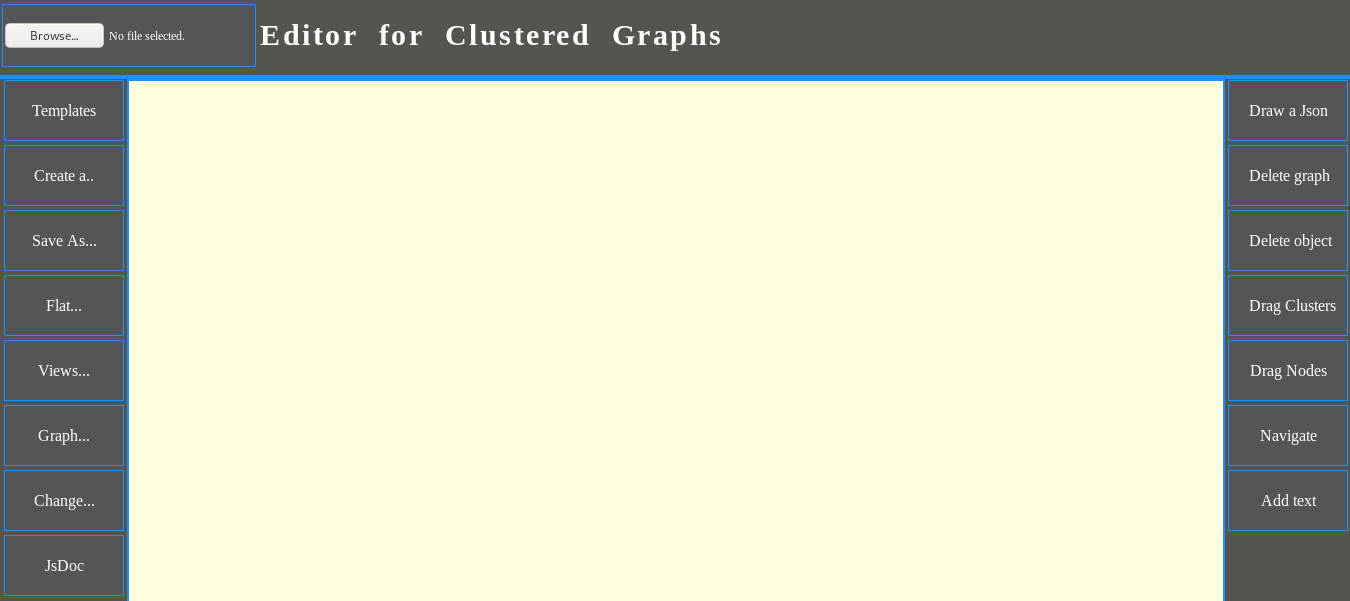
\includegraphics[width=1 \linewidth]{figure/interfaccia}
\end{center}
\caption{Log-in nel sistema\label{fig:interfaccia}}
\end{figure}
Come già accennato sarà possibile per l'utente interagire con il sistema per poter effettuare operazioni di encoding dei dati. Ogni qualvolta verrà richiesto al sistema di eseguire il log-in iniziale oppure un encode della visualizzazione il sistema risponderà con una inizializzazione. Durante la prima inzializzazione in cui sarà creata la classe \textit{clusteredGraph} e tuo ciò che ne comprende e sarà generato l'svg \#cgraph su cui si basa il piano di lavoro e con cui l'utente andrà ad interagire ed analizzare. Tutte le operazioni e le visualizzazioni saranno eseguite proprio su questo svg creato con l'ausilio della libreria grafica\textbf{ D3.js}.\\
Generato l'svg principale, sempre durante l'inizializzazione del log-iin esso verrà collegato ad altri tre oggetti svg di seguito elencati e che lo compongono:
\begin{itemize}
	\item \textbf{\#c\_cluster} che andrà a rappresentare la visualizzazione di tutti i cluster; 
	\item \textbf{\#c\_node} ovvero l'svg che rappresenta l'insieme dei nodi da visualizzare;
	\item \textbf{\#c\_edge} che rappresenterà gli archi che collegano i nodi dell'underlying graph.
\end{itemize}
La divisione degli svg che andranno a comporre quello relativo al piano di lavoro è necessaria per molteplici fattori, primo fra tutti il poter scindere una entità monolitica in molteplici oggetti è uno dei traguardi dello sviluppo software. Inoltre è possibile in questo modo poter trattare, come sarà analizzato meglio in seguito, le tre entità che rappresentano la classe \textit{ClusteredGraph} come oggetti a se stanti.\\
Una volta che l'utente ha avuto accesso al sistema ed è stato introdotto il concetto di svg e di piano di lavoro è possibile cominciare a definire quello di interfacce e di piani di lavoro diversi.
In particolare il sistema essendo basato su una coppia $<G,T>$ che compongono il grafo clusterizzato $G$ si è deciso di implementare la funzione di encode mediante la possibilità di scelta tra due viste separate viste nel dettaglio di seguito.
\section{Graph-view}
\begin{figure}[!htb]
	\begin{center}
		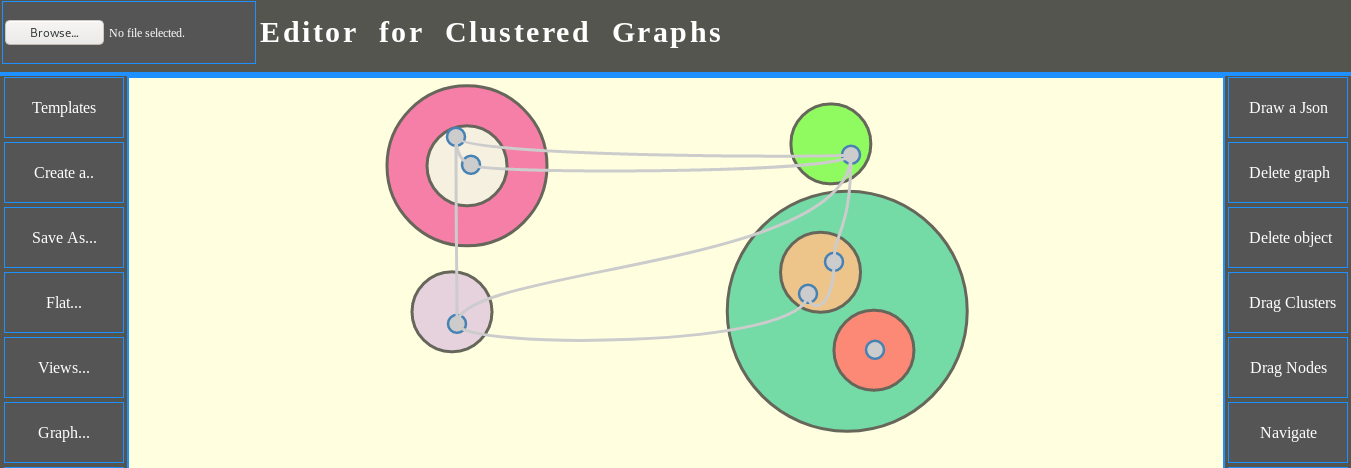
\includegraphics[width=1 \linewidth]{figure/graphView}
	\end{center}
	\caption{Graph View\label{fig:graphView}}
\end{figure}
La visualizzazione a grafo, anche definita graph-view è la visualizzazione di default ed è anche quella con cui l'utente si interfaccerà maggiormente. La graph-view è infatti l'unica vista con cui l'utente può avere una iterazione di grado tre, ovvero il grado massimo, in cui può interagire sulle modifiche e le trasformazioni non solo riguardo la visualizzazione ma anche sui dati.\\
Come si può notare dalla \figurename~\ref{fig:graphView} il modello di visualizzazione come già accennato riprende quello Node-link in cui "Node" rappresenta non solo i nodi del grafo ma anche i cluster dell'albero di inclusione. La differenza tra queste due entità a livello di visualizzazione può essere vista mediante due diversi fattori: il colore ed il raggio.
Per quanto riguarda il colore dei nodi esso risulta fisso in quanto ogni nodo rappresenterà sempre lo stesso elemento che cambierà per quanto riguarda la posizione o il cluster di appartenenza ma non nella sostanza. Anche il raggio del nodo, che verrà definito $r_n$, ha un valore fisso non dipendente da nessuna variabile.
Per quanto riguarda i cluster invece il colore, che di default presenta una randomicità nella propria visualizzazione, varia per ogni cluster definendo una ulteriore variabile che ne definisce l'unicità.
Il raggio dei cluster definito $r_c$, al contrario di quello dei nodi che come abbiamo visto è fisso esso è dipendente da variabili come sarà visto nel dettaglio ne capitolo successivo.

\section{Tree-view}
Non avendo un limite al numero di nodi e di cluster visualizzabili la graph view può ad un primo impatto portare a visualizzare un gran numero di informazioni. È facile intuire come l'occhio umano veda una rappresentazione organizzata in maniera notevolmente migliore rispetto ad una piatta e prima di profondità anche se fittizia. Per questo l'utente in qualunque momento durante una sessione di lavoro potrà interagire con il sistema e passare da una visualizzazione a grafo clusterizzato ad una dell'inclusion tree in cui però saranno rappresentati anche i nodi e gli archi dell'underlying graph.
Ogni volta che si chiederà questa operazione il sistema risponderà eliminando la visualizzazione e inizializzandone una nuova con un encode diverso degli stessi dati rappresentati in precedenza. Questa visualizzazione inizializzata sarà un svg detto \#\_ctree che possiederà grandezza uguale a quella dell' \#cgraph ma senza una divisione degli elementi che andranno a comporre la rappresentazione poichè non necessari.\\
Al contrario che nella graph view, questa risulta comunque essere un modello node-link ma in cui non si avrà necessità di inserire forze per una rappresentazione ottimale in quanto sarà una semplice rappresentazione "layered" con l'aggiunta di archi che collegano le foglie tra loro come mostrato nella \figurename~\ref{fig:treeView}.
Come si nota inoltre il raggio dei cluster e dei nodi risulta essere la stessa anche se ciò che caratterizza una foglia, che sia essa un cluster vuoto oppure un nodo all'interno di un cluster, è che questa sarà di un colore diverso rispetto ai nodi interni.
Essendo un sistema in cui non vi è una soglia massima del numero di nodi è di cluster definibili o importabili si possono presentare situazioni limite. Per questo sono state implementate due diverse tipologie di tree-view, entrambe discendenti: ad albero verticale ed orizzontale.
All'utente è lasciata la scelta di quale delle due utilizzare anche se è consigliabile ai fini di una buona visualizzazione l'utilizzo di una rappresentazione verticale nel caso in cui si hanno tanti cluster sullo stesso livello ma la profondità dell'albero è relativamente bassa mentre è sicuramente preferibile utilizzare una visualizzazione orizzonante con la radice centrale a sinistra dell'svg nel caso in cui si hanno pochi cluster per ogni livello ma una profondità maggiore da gestire.
\begin{figure}[!htb]
	\begin{center}
		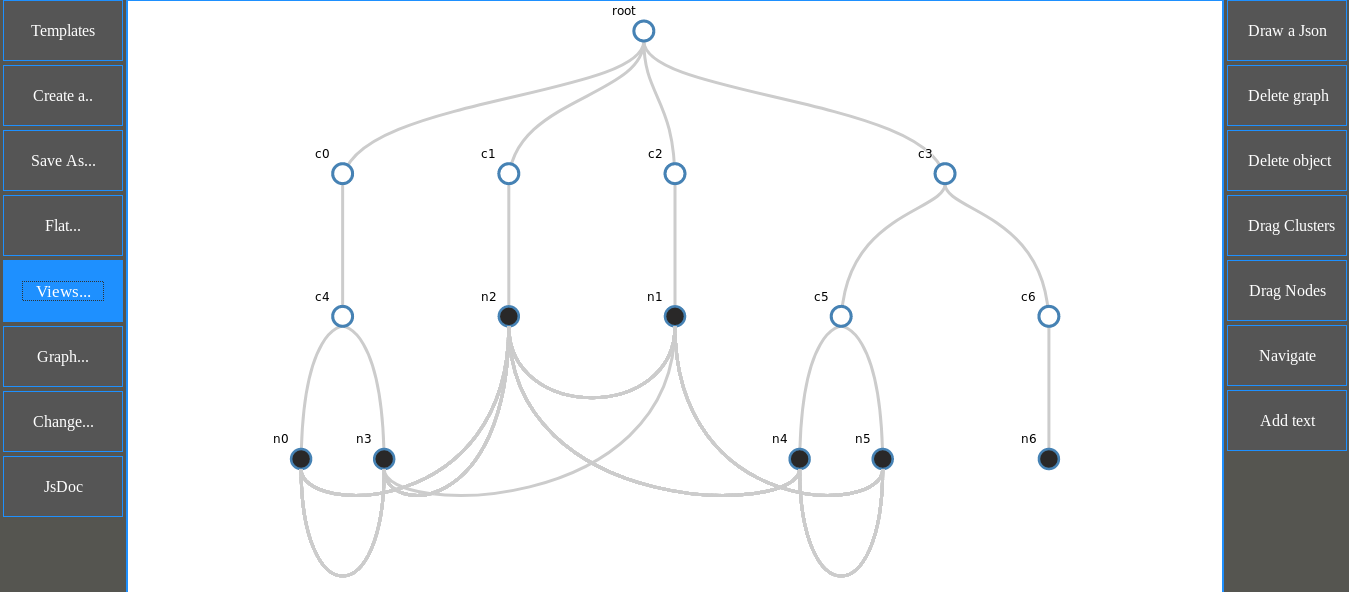
\includegraphics[width=1 \linewidth]{figure/treeView}
	\end{center}
	\caption{tree View\label{fig:treeView}}
\end{figure}
\section{Console-view}
\begin{figure}[!htb]
	\begin{center}
		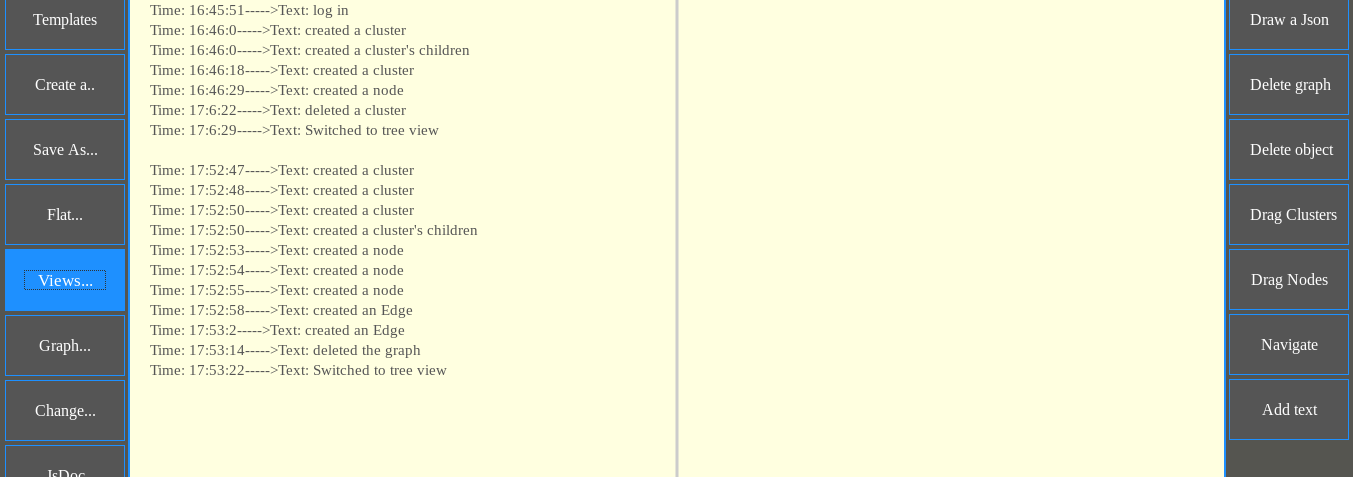
\includegraphics[width=1 \linewidth]{figure/consoleView}
	\end{center}
	\caption{Graph View\label{fig:consoleView}}
\end{figure}

\section{Filtraggio degli oggetti}
puoi mostrare solo una parte degli oggetti
\begin{figure}[!htb]
	\begin{center}
		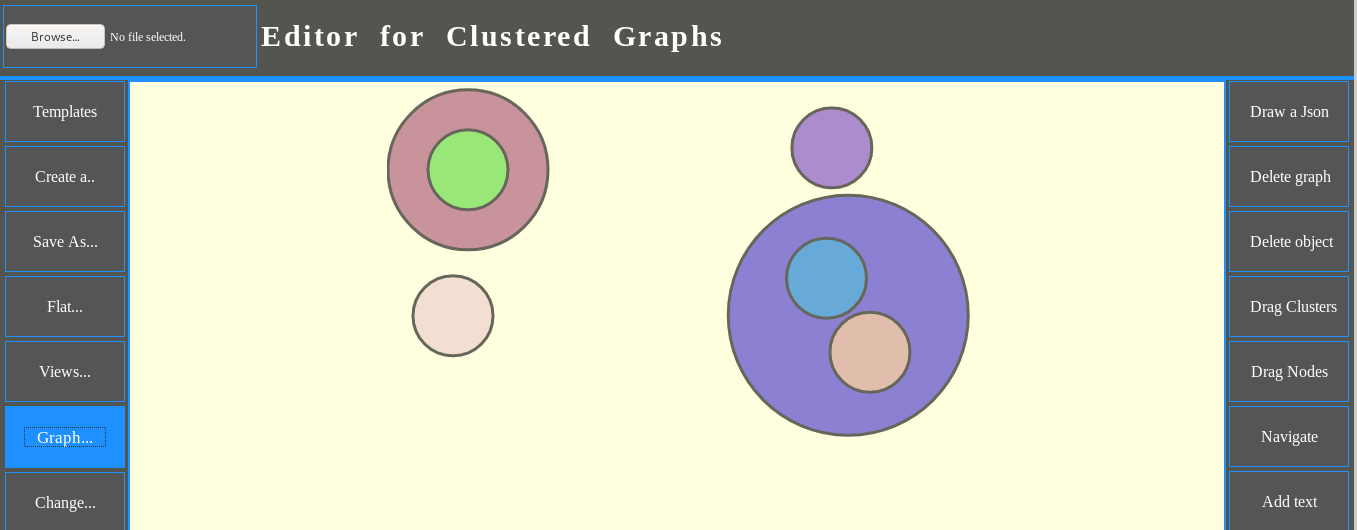
\includegraphics[width=1 \linewidth]{figure/clustersOnly}
	\end{center}
	\caption{visualizzazione dei soli cluster\label{fig:clustersOnly}}
\end{figure}

\begin{figure}[!htb]
	\begin{center}
		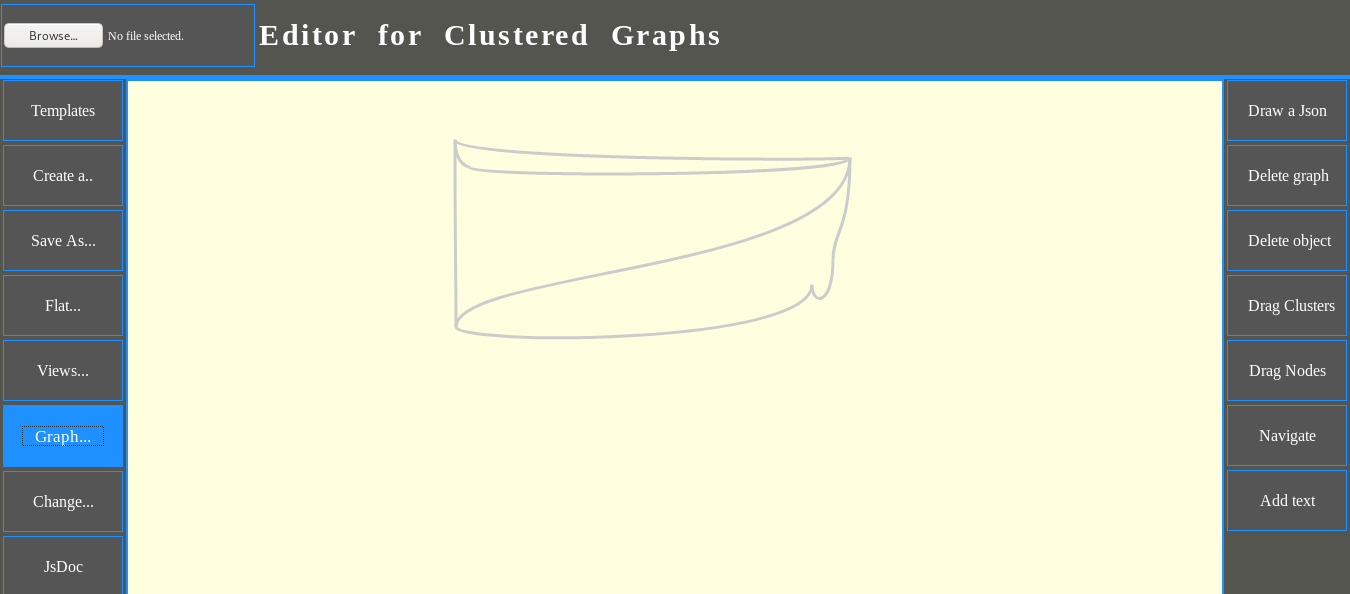
\includegraphics[width=1 \linewidth]{figure/edgesOnly}
	\end{center}
	\caption{Visualizzazione dei soli archi\label{fig:edgesOnly}}
\end{figure}

}
